\documentclass[submit]{harvardml}

\course{CS181-S22}
\assignment{Assignment \#1}
\duedate{7:59pm ET, February 4, 2022} 

\usepackage[OT1]{fontenc}
\usepackage[colorlinks,citecolor=blue,urlcolor=blue]{hyperref}
\usepackage[pdftex]{graphicx}
\usepackage{graphicx}
\usepackage{caption}
\usepackage{fullpage}
\usepackage{soul}
\usepackage{amsmath}
\usepackage{amssymb}
\usepackage{color}
\usepackage{todonotes}
\usepackage{listings}
\usepackage{common}
\usepackage{framed}
\usepackage{xcolor}

\usepackage[mmddyyyy,hhmmss]{datetime}

\definecolor{verbgray}{gray}{0.9}

\newcommand{\Lagr}{\mathcal{L}}

\lstnewenvironment{csv}{
  \lstset{backgroundcolor=\color{verbgray},
  frame=single,
  framerule=0pt,
  basicstyle=\ttfamily,
  columns=fullflexible}}{}
 

\begin{document}
\begin{center}
{\Large Homework 1: Regression}\\
\end{center}

\subsection*{Introduction}
This homework is on different forms of linear regression and focuses
on loss functions, optimizers, and regularization. Linear regression
will be one of the few models that we see that has an analytical
solution.  These problems focus on deriving these solutions and
exploring their properties.

If you find that you are having trouble with the first couple
problems, we recommend going over the fundamentals of linear algebra
and matrix calculus (see links on website).  The relevant parts of the
\href{https://github.com/harvard-ml-courses/cs181-textbook/blob/master/Textbook.pdf}{cs181-textbook notes are Sections 2.1 - 2.7}.  We strongly recommend
reading the textbook before beginning the homework.

    We also encourage you to first read the \href{http://users.isr.ist.utl.pt/~wurmd/Livros/school/Bishop\%20-\%20Pattern\%20Recognition\%20And\%20Machine\%20Learning\%20-\%20Springer\%20\%202006.pdf}{Bishop textbook}, particularly:
Section 2.3 (Properties of Gaussian Distributions), Section 3.1
(Linear Basis Regression), and Section 3.3 (Bayesian Linear
Regression). (Note that our notation is slightly different but the
underlying mathematics remains the same!).

\textbf{Please type your solutions after the corresponding problems using this
\LaTeX\ template, and start each problem on a new page.} You may find
the following introductory resources on \LaTeX\ useful: 
\href{http://www.mjdenny.com/workshops/LaTeX_Intro.pdf}{\LaTeX\ Basics} 
and \href{https://www.overleaf.com/learn/latex/Free_online_introduction_to_LaTeX_(part_1)}{\LaTeX\ tutorial with exercises in Overleaf}

Homeworks will be submitted through Gradescope. You will be added to
the course Gradescope once you join the course Canvas page. If you
haven't received an invitation, contact the course staff through Ed.

\textbf{Please submit the writeup PDF to the Gradescope assignment
  `HW1'.} Remember to assign pages for each question.

\textbf{Please submit your \LaTeX file and code files to the
  Gradescope assignment `HW1 - Supplemental'.} Your files should be
named in the same way as we provide them in the repository,
e.g. \texttt{T1\_P1.py}, etc.


%%%%%%%%%%%%%%%%%%%%%%%%%%%%%%%%%%%%%%%%%%%%%
% Problem 1
%%%%%%%%%%%%%%%%%%%%%%%%%%%%%%%%%%%%%%%%%%%%%

\begin{problem}[Optimizing a Kernel, 15pts]

Kernel-based regression techniques are similar to nearest-neighbor
regressors: rather than fit a parametric model, they predict values
for new data points by interpolating values from existing points in
the training set.  In this problem, we will consider a kernel-based
regressor of the form:
\begin{equation*}
  f(x^*) = \sum_{n} K(x_n,x^*) y_n 
\end{equation*}
where $(x_n,y_n)$ are the training data points, and $K(x,x')$ is a
kernel function that defines the similarity between two inputs $x$ and
$x'$. Assume that each $x_i$ is represented as a column vector, i.e. a
$D$ by 1 vector where $D$ is the number of features for each data
point. A popular choice of kernel is a function that decays as the
distance between the two points increases, such as
\begin{equation*}
  K(x,x') = \exp\left(\frac{-||x-x'||^2_2}{\tau}\right) = \exp\left(\frac{-(x-x')^T (x-x')}{\tau} \right) 
\end{equation*}
where $\tau$ represents the square of the lengthscale (a scalar value).  In this
problem, we will consider optimizing what that (squared) lengthscale
should be.

\begin{enumerate}

\item Let $\{(x_n,y_n)\}_{n=1}^N$ be our training data set.  Suppose
  we are interested in minimizing the residual sum of squares.  Write
  down this loss over the training data $\mcL(W)$ as a function of $\tau$.

  Important: When computing the prediction $f(x_i)$ for a point $x_i$
  in the training set, carefully consider for which points $x'$ you should be including
  the term $K(x_i,x')$ in the sum.

\item Take the derivative of the loss function with respect to $\tau$.
\end{enumerate}

\end{problem}

\newpage

\begin{framed}
\noindent\textbf{Problem 1} (cont.)\\

\begin{enumerate}
\setcounter{enumi}{2}
\item Consider the following data set:
\begin{csv}
  x , y
  0 , 0
  1 , 0.5
  2 , 1
  3 , 2
  4 , 1
  6 , 1.5
  8 , 0.5 
\end{csv}
And the following lengthscales: $\tau=.01$, $\tau=2$, and $\tau=100$.

Write some Python code to compute the loss with respect to each kernel
for the dataset provided above. Which lengthscale does best?  
For this problem, you can use our staff \textbf{script to compare your
  code to a set of staff-written test cases.} This requires, however,
that you use the structure of the starter code provided in
\texttt{T1\_P1.py}. More specific instructions can be found at the top
of the file \texttt{T1\_P1\_Testcases.py}. You may run the test cases
in the command-line using \texttt{python T1\_P1\_TestCases.py}.
\textbf{Note that our set of test cases is not comprehensive: just
  because you pass does not mean your solution is correct! We strongly
  encourage you to write your own test cases and read more about ours
  in the comments of the Python script.}
  
\item Plot the function $(x^*, f(x^*))$ for each of the
  lengthscales above.  You will plot $x^*$ on the x-axis and the
  prediction $f(x^*)$ on the y-axis.  For the test inputs $x^*$, you
  should use an even grid of spacing of $0.1$ between $x^* = 0$ and
  $x^* = 12$.  (Note: it is possible that a test input $x^*$ lands
  right on top of one of the training inputs above.  You can still use
  the formula!) 

  Initial impressions: Briefly describe what happens in each of the
  three cases.  Is what you see consistent with the which lengthscale
  appeared to be numerically best above?  Describe why or why not.

\item Bonus: Code up a gradient descent to optimize the kernel for the
  data set above.
  Start your gradient descent from $\tau=2$. Report on what you
  find.\\\\

  Note: Gradient descent is discussed in Section 3.4 of the
  cs181-textbook notes and Section 5.2.4 of Bishop, and will be
  covered later in the course!

\end{enumerate}
  
\end{framed}  

\newpage
\textcolor{blue}{
\begin{framed}
Solutions
\begin{enumerate}
    \item The loss function here will be:
            \begin{equation*}
              \Lagr(\tau) = \sum_{n=1}^N (y_n - \sum_{i=1, i \neq n}^N \exp\left(\frac{-||x_n-x_i||^2_2}{\tau}\right) y_i)^2 
            \end{equation*}
        We don't want to include the $i=n$ case in the inner sum, as we want to include our best guess for $y$, and if $y$ is already in the training set, it defeats the purpose for training on that point.
    \item With $\Lagr(\tau)$ as defined above:
        \begin{equation*}
            \frac{\partial \Lagr}{\partial \tau} = 
            -2\sum_{n=1}^N ((y_n - \sum_{i=1, i \neq n}^N \exp\left(\frac{-||x_n-x_i||^2_2}{\tau}\right) y_i)
            (\sum_{i=1, i \neq n}^N \frac{||x_n-x_i||_2^2}{\tau^2}\exp\left(\frac{-||x_n-x_i||^2_2}{\tau}\right)y_i))
        \end{equation*}
    \item The loss for $\tau$ = 0.01 is 8.75, loss for $\tau$ = 2: 3.305, and loss for $\tau$ = 100: 120.359. It seems here that the value of $\tau = 2$ did the best, as the loss is minimized in this case.
    \item The plots are below: \newline
    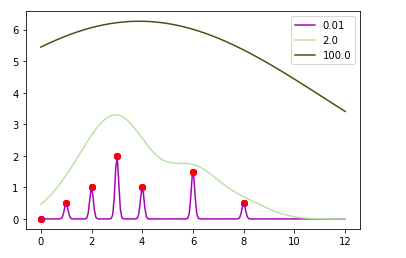
\includegraphics[]{1.3.png}
    \newline In general, for all of these cases, higher the $\tau$, more we overestimate, because the method we use is not normalized. \newline We see that for the $\tau = 0.1$ case, there is a lot of "overfitting" happening, in that the model is extremely accurate for values close to the training data, but not otherwise. This is because the kernel decays exponentially in regards to error, so the points that are not close to the training data have extremely low values due to this. \newline In the $\tau = 2$ case, we see that this is a much better fit to the data, even though it is overestimated, as the $\tau$ used here is such that the decay function doesn't decay too fast or too slow as we move away from training data. \newline In the $\tau = 100.0$ case, there is a lot of smoothing, as the kernel weighs distant points too much. As such, it is not a good fit.
\end{enumerate}
\end{framed}
}
\newpage

%%%%%%%%%%%%%%%%%%%%%%%%%%%%%%%%%%%%%%%%%%%%%
% Problem 2
%%%%%%%%%%%%%%%%%%%%%%%%%%%%%%%%%%%%%%%%%%%%%

\begin{problem}[Kernels and kNN, 10pts]

Now, let us compare the kernel-based approach to an approach based on
nearest-neighbors.  Recall that kNN uses a predictor of the form
  \begin{equation*}
    f(x^*) = \frac{1}{k} \sum_n y_n \mathbb{I}(x_n \texttt{ is one of k-closest to } x^*)
  \end{equation*}

\noindent where $\mathbb{I}$ is an indicator variable. For this problem, you will use the \textbf{same dataset and kernel as in Problem 1}.


For this problem, you can use our staff \textbf{script to compare your code to a set of staff-written test cases.} This requires, however, that you use the structure of the starter code provided in \texttt{T1\_P2.py}. More specific instructions can be found at the top of the file \texttt{T1\_P2\_Testcases.py}. You may run the test cases in the command-line using \texttt{python T1\_P2\_TestCases.py}.
\textbf{Note that our set of test cases is not comprehensive: just because you pass does not mean your solution is correct! We strongly encourage you to write your own test cases and read more about ours in the comments of the Python script.}

\vspace{0.5cm}
\noindent\emph{Make sure to include all required plots in your PDF.}


\begin{enumerate}

\item Implement kNN for $k=\{1, 3, N-1\}$ where N is the size of the dataset, then plot the results for each $k$. To find the distance between points, use the kernel function from Problem 1 with lengthscale $\tau=1$. 

As before, you will plot $x^*$ on the x-axis and the prediction $f(x^*)$ on the y-axis.  For the test inputs $x^*$, you should use an even grid of spacing of $0.1$ between $x^* = 0$ and $x^* = 12$.  (Like in Problem 1, if a test point lies on top of a training input, use the formula without excluding that training input.)
  
  You may choose to use some starter Python code to create your plots
  provided in \verb|T1_P2.py|.  Please \textbf{write your own
    implementation of kNN} for full credit.  Do not use external
  libraries to find nearest neighbors.
  
\item Describe what you see: What is the behavior of the functions in
  these three plots?  How does it compare to the behavior of the
  functions in the three plots from Problem 1?  Are there situations
  in which kNN and kernel-based regression interpolate similarly?
  Extrapolate similarly?  Based on what you see, do you believe there
  exist some values of $k$ and $\tau$ for which the kNN and kernel-based regressors produce the exact same classifier (ie. given \textit{any} point $x$, the two regressors will produce the same prediction $f(x)$)? Explain your answer.
  
\item Why did we not vary $\tau$ for the kNN approach?

\end{enumerate}

\end{problem}

\newpage
\textcolor{blue}{
\begin{framed}
Solutions
\begin{enumerate}
    \item The plots for all are below, with code in the supplemental. \newline
    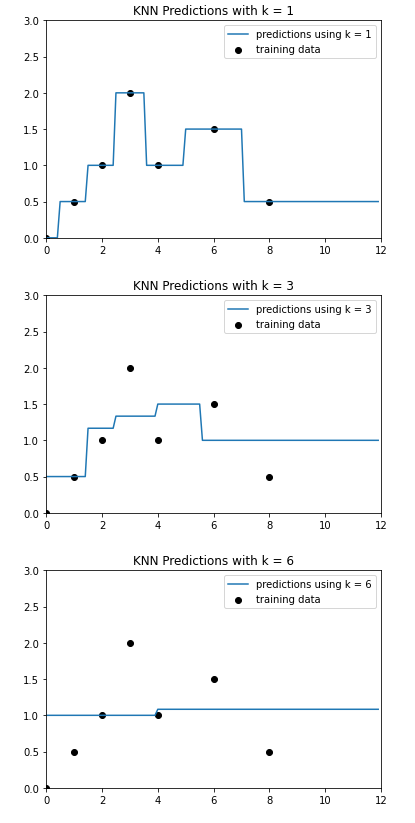
\includegraphics[scale=0.5]{2.1_plots.png}
    \item \textcolor{blue}{For the $k=1$ predictor, we see that it just fits the nearest point, so it doesn't average at all. For the $k=3$ predictor, we can see that it averages better than the k=1 predictor, so it "stays between" the points more. Lastly, for the $k=N-1$ predictor, it is at all times extremely close to the sample mean, as it averages all but one of the points.\newline \\  Regarding extrapolation and interpolation, the kNN and Kernel Regressor models don't seem to be similar. For the former, see that in kNN, we predict either the averages of the last $k$ points as x trends towards infinity, or the average of the first $k$ points as x trends towards negative infinity. Unless the average of these points is 0, this prediction will not be zero. In the kernel regressor, as x trends towards infinity and negative infinity, we will trend towards zero, as the kernel function trends towards 0 as the distance from the input $x*$ to the training data $x$ grows to infinity. In regards to interpolation, see that the kNN model averages out the high / low value data points, while the kernel formula "peaks" and favors these high / low value data points (as we see when the predicted input is a training input). I guess in some sense, the $\tau=2$ and $k = 1$ case do look similar (except one is discrete, another is continuous, and we don't normalize in the kernel regressor), though the similarities are limited. \newline \\ 
    I don't think that there exists some values of $k, \tau$, such that the kNN and kernel based regressor produce the exact same classifier. First off, kNN classifiers aren't smooth, and have some discrete steps in the prediction as we see in our graphs, unlike kernel regressors which are. In addition, as we said before, kNN averages, avoiding predictions that are extremely high or low, while kernel regressor predicts based on these peaks. One case I can think of where there could perhaps exist some value of $k$ or $\tau$ such that the predictors are very, very similar, is if the data is basically defined for all $x \in \mathbb{R}$ - in this case, $k = 1$, and a very small $\tau$ might converge to the same plot, though I am not sure (this might require some real analysis).}
    \item The reason we didn't vary $\tau$ is because kNN only depends on the $k$-closest to $x^*$. If we look at the distance function we used, it is exponential, which is monotonically increasing. In addition, since the negative L2-norm is what we input to the distance function, as long as $\tau$ is positive, changing $\tau$ does not affect the relative closeness of points to other points, so the $k$ closest neighbors for any input point will be the same regardless of $\tau$.
\end{enumerate}
\end{framed}
}
\newpage 

%%%%%%%%%%%%%%%%%%%%%%%%%%%%%%%%%%%%%%%%%%%%%
% Problem 3
%%%%%%%%%%%%%%%%%%%%%%%%%%%%%%%%%%%%%%%%%%%%%

\begin{problem}[Deriving Linear Regression, 10pts]

  The solution for the least squares linear regressions ``looks'' kind
  of like a ratio of covariance and variance terms.  In this problem,
  we will make that connection more explicit. \\

  \noindent Let us assume that our data are tuples of scalars $(x,y)$ that are
  described by some joint distribution $p(x,y)$.  For clarification, the joint distribution $p(x,y)$ is just another way of saying the ``joint PDF'' $f(x,y)$, which may be more familiar to those who have taken Stat 110, or equivalent. \\
  
  \noindent We will consider the process of fitting these data from this distribution with the best linear model
  possible, that is a linear model of the form $\hat{y} = wx$ that
  minimizes the expected squared loss $E_{x,y}[ ( y - \hat{y} )^2
  ]$.\\

\noindent \emph{Notes:} The notation $E_{x, y}$ indicates an
expectation taken over the joint distribution $p(x,y)$.  Since $x$ and
$y$ are scalars, $w$ is also a scalar.
  
  \begin{enumerate}

  \item Derive an expression for the optimal $w$, that is, the $w$
    that minimizes the expected squared loss above.  You should leave
    your answer in terms of moments of the distribution, e.g. terms
    like $E_x[x]$, $E_x[x^2]$, $E_y[y]$, $E_y[y^2]$, $E_{x,y}[xy]$
    etc.

\item Provide unbiased and consistent formulas to estimate $E_{x, y}[yx]$
 and $E_x[x^2]$ given observed data $\{(x_n,y_n)\}_{n=1}^N$.

\item In general, moment terms like $E_{x, y}[yx]$, $E_{x, y}[x^2]$,
  $E_{x, y}[yx^3]$, $E_{x, y}[\frac{x}{y}]$, etc. can easily be
  estimated from the data (like you did above).  If you substitute in
  these empirical moments, how does your expression for the optimal
  $w^*$ in this problem compare with the optimal $w^*$ that we see in
  Section 2.6 of the cs181-textbook?

\item Many common probabilistic linear regression models assume that
  variables x and y are jointly Gaussian.  Did any of your above
  derivations rely on the assumption that x and y are jointly
  Gaussian?  Why or why not?
    
\end{enumerate}

\end{problem}


\newpage
\textcolor{blue}{
\begin{framed}
Solution 3
\begin{enumerate}
    \item The optimal $w = \frac{\mathbb{E}_x_y(xy)}{\mathbb{E}_x(x^2)}$, as shown below:
        \begin{gather*}
            \Lagr(w) = \mathbb{E}_x_y(y-\hat{y})^2 \\
            = \mathbb{E}_x_y(y-wx)^2 \\ 
            = \mathbb{E}_x_y(y^2-2wxy-w^2x^2 \\ 
            = \mathbb{E}_y(y^2) + 2w\mathbb{E}_x_y(xy) + w^2\mathbb{E}_x(x^2)
        \end{gather*}
    The last step is by linearity of expectations. Then, we minimize $\Lagr(w)$ by differentiating in respect to w and setting to zero. 
        \begin{gather*}
            \frac{d\Lagr}{d w} = 2w\mathbb{E}_x(x^2) - 2\mathbb{E}_x_y(xy) \\
            0 = 2w*\mathbb{E}_x(x^2) - 2\mathbb{E}_x_y(xy) \\
            w* = \frac{\mathbb{E}_x_y_(xy)}{\mathbb{E}_x(x^2)}
        \end{gather*}
    See that this is a minimum by the second derivative test, since $\mathbb{E}_x(x^2) \geq 0$
        \begin{gather*}
            \frac{d^2 \Lagr}{dw^2} = 2\mathbb{E}_x(x^2)
        \end{gather*}
    \item We can estimate these by using the sample mean:
        \begin{gather*}
            \mathbb{E}_x_y(xy) \approx \frac{1}{N} \sum_n x_n y_n \\
            \mathbb{E}_x(x^2) \approx \frac{1}{N} \sum_n x_n^2
        \end{gather*}
    \item Plugging in our estimations above, and having X be the "design matrix" for x, and Y be the one dimensional vector of outputs y (one dimensional), we see that 
        \begin{gather*}
            w^* = \frac{\mathbb{E}_x_y_(xy)}{\mathbb{E}_x(x^2)} \\
            \approx \frac{\frac{1}{N} \sum_n x_n y_n}{\frac{1}{N} \sum_n x_n^2} \\
            = \frac{\sum_n x_n y_n}{\sum_n x_n^2}
            = \frac{XY^T}{XX^T}
            = (X^TX)^{-1}(X^Ty)
        \end{gather*}
        This is the same as the optimal $w^*$ we see in section 2.6!
    \item None of the assumptions made above assume that variables x and y are jointly Gaussian, as we assumed that $p(x,y)$ is the pdf of any distribution.
\end{enumerate}
\end{framed}
}
\newpage

%%%%%%%%%%%%%%%%%%%%%%%%%%%%%%%%%%%%%%%%%%%%%
% Problem 4
%%%%%%%%%%%%%%%%%%%%%%%%%%%%%%%%%%%%%%%%%%%%%

\begin{problem}[Modeling Changes in Republicans and Sunspots, 15pts]
  
 The objective of this problem is to learn about linear regression
 with basis functions by modeling the number of Republicans in the
 Senate. The file \verb|data/year-sunspots-republicans.csv| contains the
 data you will use for this problem.  It has three columns.  The first
 one is an integer that indicates the year.  The second is the number
 of Sunspots observed in that year.  The third is the number of Republicans in the Senate for that year.
 The data file looks like this:
 \begin{csv}
Year,Sunspot_Count,Republican_Count
1960,112.3,36
1962,37.6,34
1964,10.2,32
1966,47.0,36
\end{csv}

You can see scatterplots of the data in the figures below.  The horizontal axis is the Year, and the vertical axis is the Number of Republicans and the Number of Sunspots, respectively.

\begin{center}
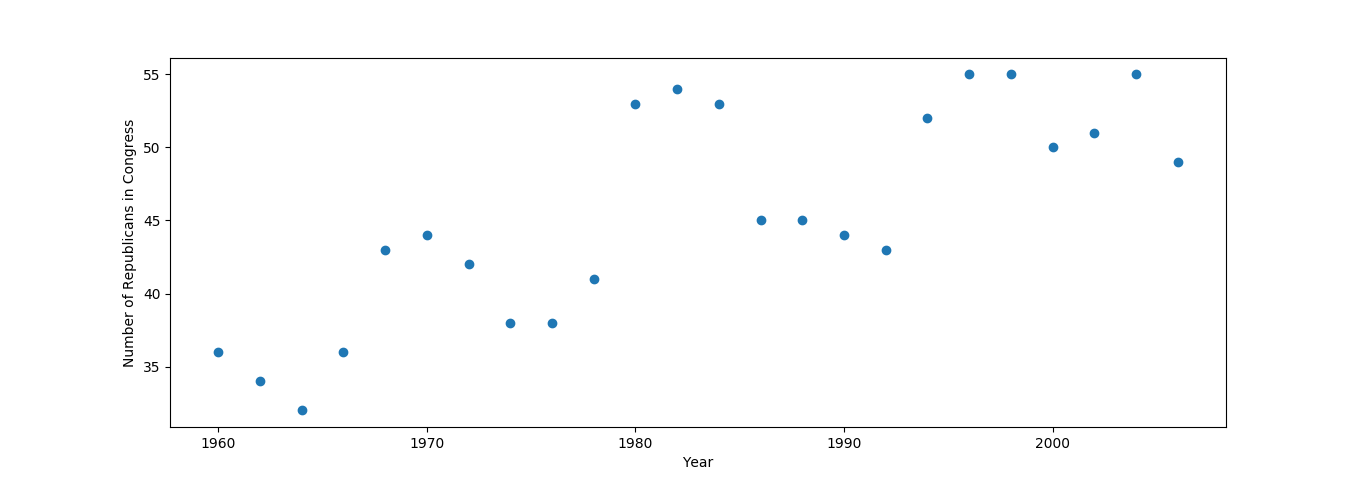
\includegraphics[width=.5\textwidth]{data/year-republicans}
\end{center}

\begin{center}
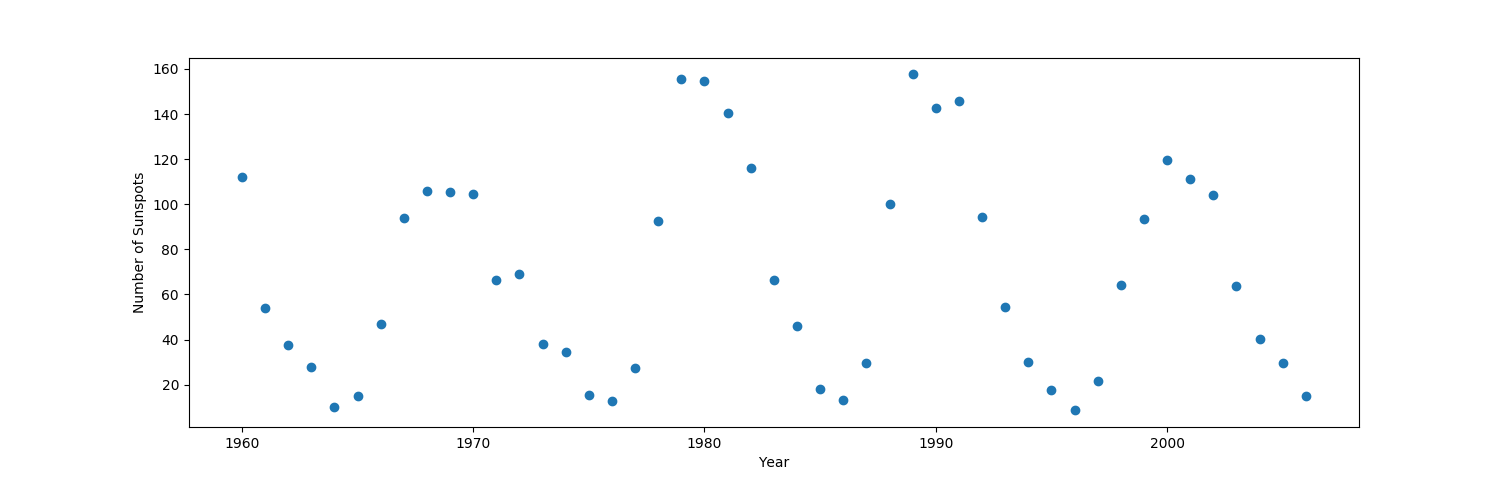
\includegraphics[width=.5\textwidth]{data/year-sunspots}
\end{center}

(Data Source: \url{http://www.realclimate.org/data/senators_sunspots.txt})\\
\vspace{-5mm}


\vspace{0.5cm}
\noindent\emph{Make sure to include all required plots in your PDF.}

\begin{enumerate}

\item In this problem you will implement ordinary least squares
  regression using 4 different basis functions for \textbf{Year
    (x-axis)} v. \textbf{Number of Republicans in the Senate
    (y-axis)}. Some starter Python code that implements simple linear
  regression is provided in \verb|T1_P4.py|.

  Note: The numbers in the \emph{Year} column are large (between $1960$ and $2006$), especially when raised to various powers. To avoid numerical instability due to ill-conditioned matrices in most numerical computing systems, we will scale the data first: specifically, we will scale all ``year'' inputs by subtracting $1960$ and then dividing by $40$. Similarly, to avoid numerical instability with numbers in the \emph{Sunspot\_Count} column, we will also scale the data first by dividing all ``sunspot count'' inputs by $20$. Both of these scaling procedures have already been implemented in lines $65-69$ of the starter code in \verb|T1_P4.py|. Please do \emph{not} change these lines!

First, plot the data and regression lines for each of the following sets of basis functions, and include
the generated plot as an image in your submission PDF. You will therefore make 4 total plots:
\begin{enumerate}
	\item[(a)] $\phi_j(x) = x^j$ for $j=1, \ldots, 5$\\
    ie, use basis $y = a_1 x^1 + a_2 x^2 + a_3 x^3 + a_4 x^4 + a_5 x^5$ for some constants $\{a_1, ..., a_5\}$. 
    \item[(b)] $\phi_j(x) = \exp{\frac{-(x-\mu_j)^2}{25}}$ for $\mu_j=1960, 1965, 1970, 1975, \ldots 2010$
	\item[(c)] $\phi_j(x) = \cos(x / j)$ for $j=1, \ldots, 5$
	\item[(d)] $\phi_j(x) = \cos(x / j)$ for $j=1, \ldots, 25$
\end{enumerate}
\vspace{-2mm}


{\footnotesize * Note: Please make sure to add a bias term for all your basis functions above in your implementation of the \verb|make_basis| function in \verb|T1_P4.py|.}
  
Second, for each plot include the residual sum of squares error. Submit the generated plot and residual sum-of-squares error for each basis in your LaTeX write-up.
\end{enumerate}

\end{problem}

\begin{framed}
\noindent\textbf{Problem 4} (cont.)\\
\begin{enumerate}
\setcounter{enumi}{1}
\item Repeat the same exact process as above but for \textbf{Number of Sunspots (x-axis)} v. \textbf{Number of Republicans in the Senate (y-axis)}. 
Now, however, only use data from before 1985, and only use basis functions (a), (c), and (d) -- ignore basis (b). You will therefore make 3 total plots. For each plot make sure to also include the residual sum of squares error.



Which of the three bases (a, c, d) provided the "best" fit? \textbf{Choose one}, and keep in mind the generalizability of the model. 

Given the quality of this fit, do you believe that the number of sunspots controls the number of Republicans in the senate (Yes or No)?
\end{enumerate}
\end{framed}

\newpage
\textcolor{blue}{
\begin{framed}
Solution 4
\begin{enumerate}
    \item Below are both the data and regression lines for each of the sets of basis functions, and the residual sum of squares error. \newline
    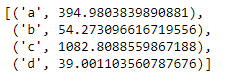
\includegraphics[scale = 1]{4.1_year_errors.png} \newline
    \includegraphics[scale = 0.55]{4.1_plots.png} \newline
    \item Below are the data and regression lines for each of the set of basis functions for the second part, as well as squared error. 
    \newline
    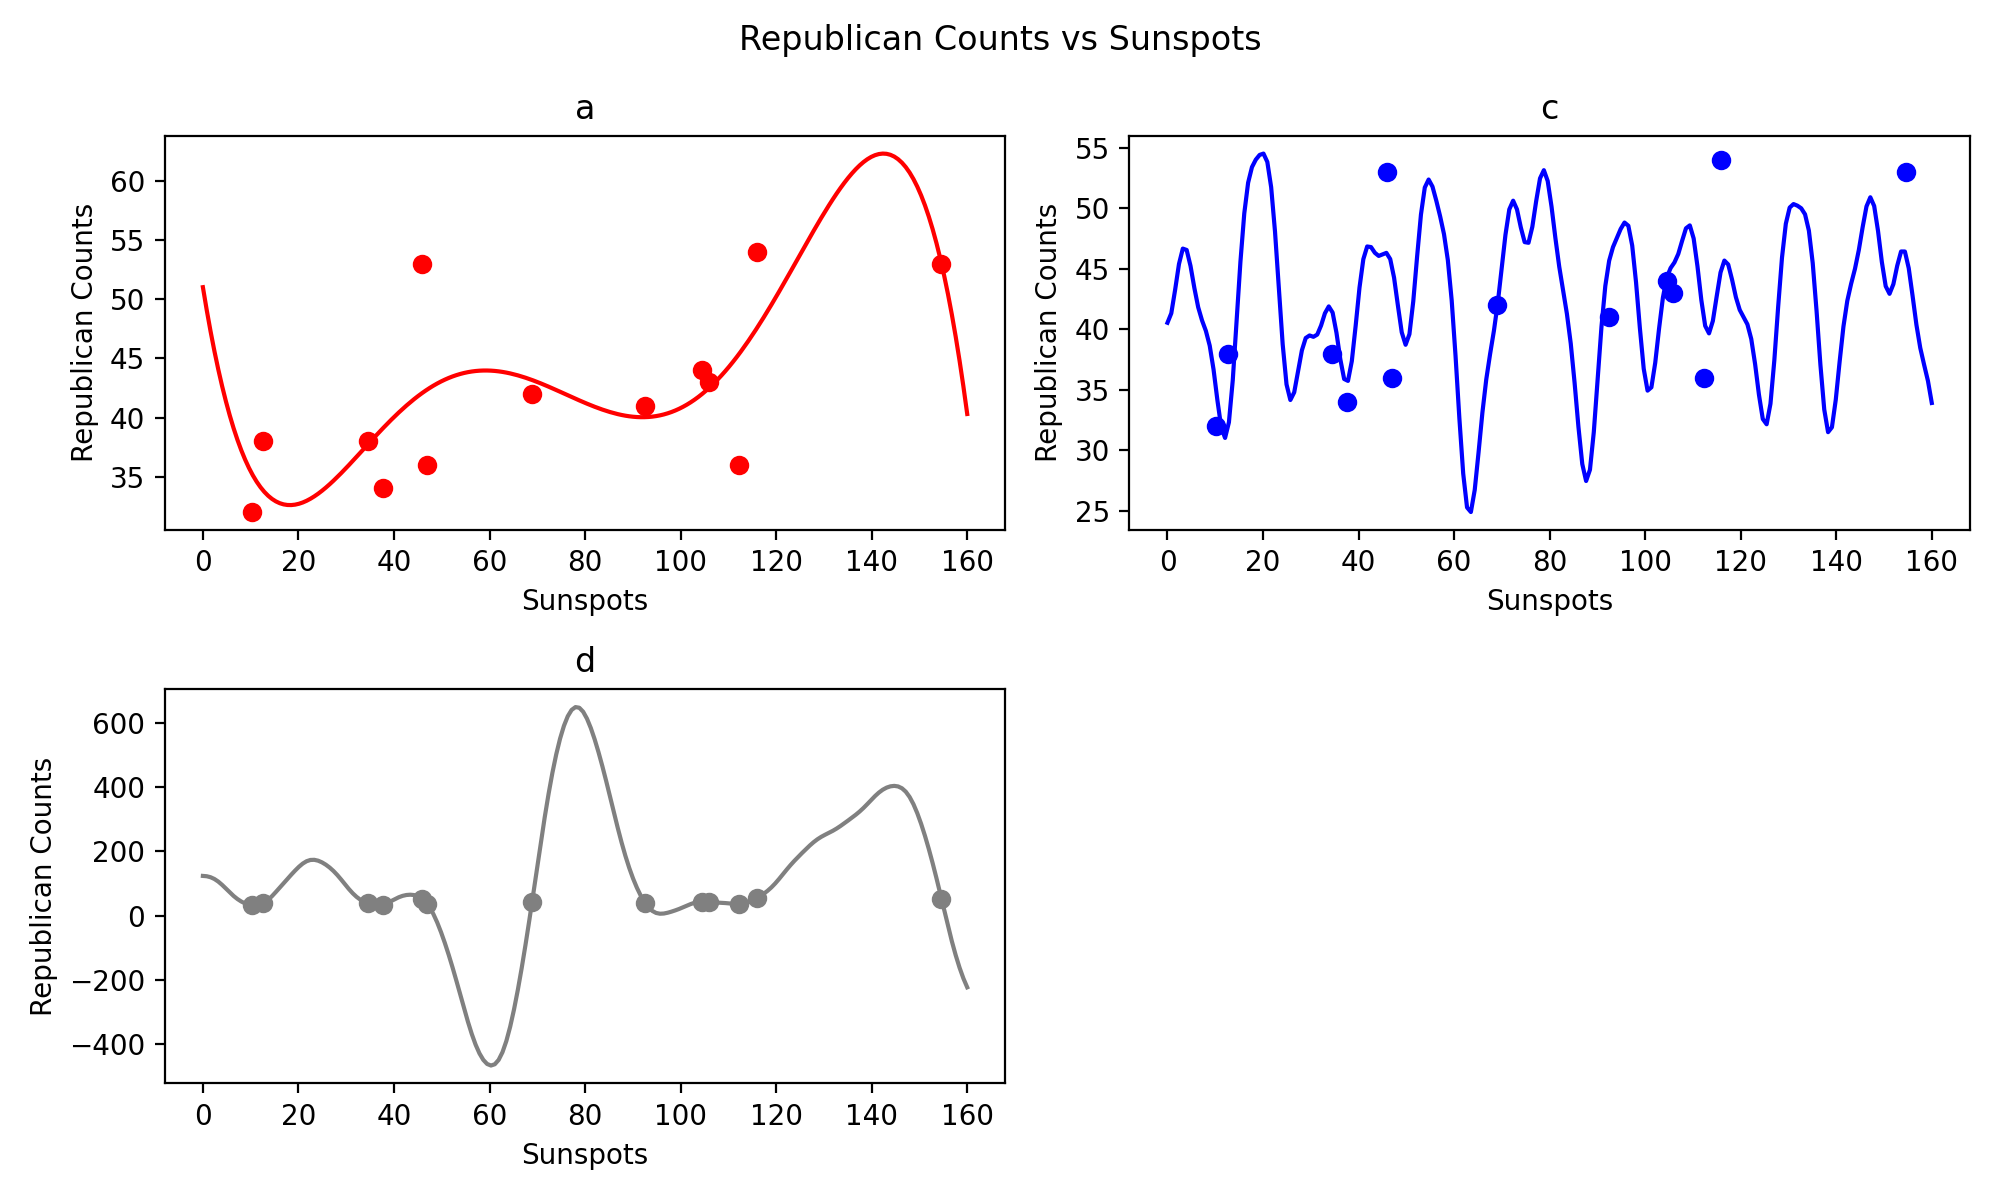
\includegraphics[scale = 0.55]{PS1_P4_countsvssunspots.png}
    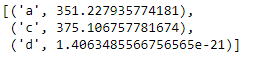
\includegraphics[]{4.2_errors.png}
    \newline
    The best "fit" (lowest squared error) came from the model fit with basis d. However, it is not generalizable - it is impossible that at around 60 sunspots, we'd predict -400 as the count of Republicans. It is likely that this is the best fit because we overfit with 25 dimensions for $w$. For basis c, this is clearly not generalizable as well, given the abrupt spikes between data points. As such, we are left with basis a, which doesn't do the best in terms of loss, but at least doesn't jump to extremes, and is relatively smooth in between the domain of sunspots that we've seen. \newline  It is important to note that we are talking about interpolation here, as extrapolation wise, none of these functions seems to do a great job (a would diverge, c and d would be periodic with the same issues that interpolation brought). Given the quality of the fit, I am not convinced that the number of spots control the number of Republicans in the Senate. Intuitively, that doesn't make any sense. Qualitatively, looking at the graph, it seems like the correlation is near zero, and what is there is just noise - the curve we fit seems pretty arbitrary, but "good" enough that it looks like it fits.
\end{enumerate}
\end{framed}
}


\newpage
%%%%%%%%%%%%%%%%%%%%%%%%%%%%%%%%%%%%%%%%%%%%%
% Name and Calibration
%%%%%%%%%%%%%%%%%%%%%%%%%%%%%%%%%%%%%%%%%%%%%
\subsection*{Name}

John Wang 

\subsection*{Collaborators and Resources}
Whom did you work with, and did you use any resources beyond cs181-textbook and your notes?

Josh Michels, Leonard Tang

\subsection*{Calibration}
Approximately how long did this homework take you to complete (in hours)? 

15 hours


\end{document}